\pagestyle{fancy}
\renewcommand{\theUnit}{5}
\ifthenelse{\isundefined{\UnitPageNumbers}}{}{\setcounter{page}{1}}
\rhead{Chapter \theUnit: Bootstrap Distributions}
\lhead{Math 3382: Statistical Theory}
%\lhead{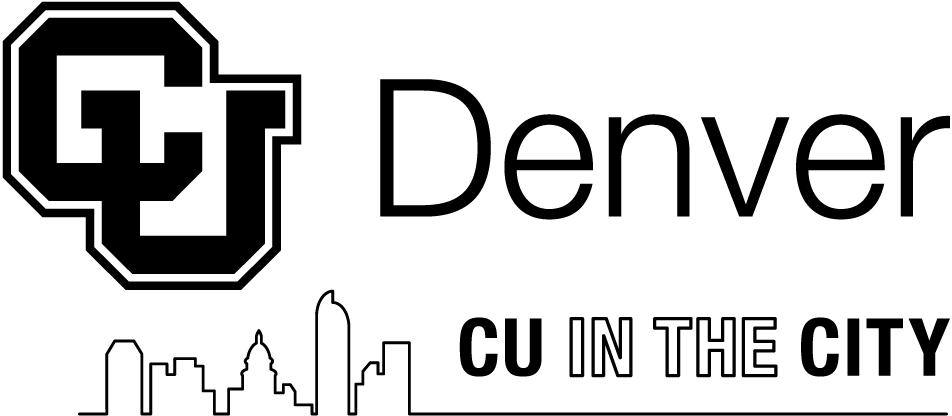
\includegraphics[width=1.25cm]{CUDenver-Logo.png}}
\rfoot{\mypage}
\cfoot{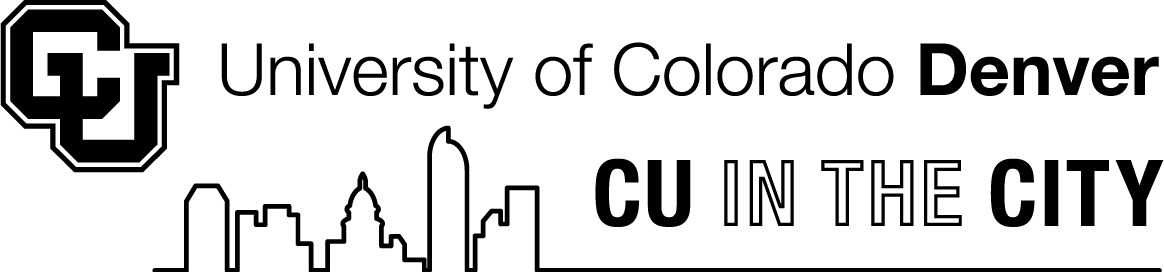
\includegraphics[width=2.25cm]{CUDenver-Logo-coverpage.png}}
\lfoot{Adam Spiegler}
\fancypagestyle{firstfooter}{\footskip = 50pt}
\renewcommand{\footrulewidth}{.4pt}
%%%%%%%%%%%%%%%%%%%%%%%%%%%
\vspace*{-20pt} \thispagestyle{firstfooter}


%\begin{tasks}[counter-format = {(tsk[a])},label-offset = {0.8em},label-format = {\color{black}\bfseries}](2)

\pagebegin{Chapter 5: Bootstrap Distributions}

A common feature of previous examples is that the distribution for the population(s) was known.
\bi
\ii For example if a coin is fair, then we know the population is binomial with $p=0.5$, and we can answer questions about the probability of certain events occurring.
\ii If we have population $X \sim \mbox{Exp} ( \lambda )$, then we can use CLT to calculate $P( \overline{X} < 10 )$.
\ei

\bbox
What if the population is unknown? When we use data from a sample to describe some characteristic of the population, we are doing statistics!
\bi
\ii A \textbf{\colorb{parameter}} is a characteristic of a population (which may be a probability distribution).
\ii A \textbf{\colorb{statistic}} is a characteristic of a sample.
\ii A parameter is a typically a number (mean, proportion, ratio of two means) that is unknown.
\ii Recall we use different notation for parameters and statistics.
\ii Statistic(s) from a sample can be used to estimate unknown population parameter(s).
\ei
\ebox


\bb
\ii  Imagine you would like to answer the following question?

\begin{center}\textbf{``What is the average weight of all babies that were born this past year?''}\end{center}

How could you go about answering this question?


\ee

\clearpage

\pagebegin{Estimating the Weight of All Newborns}


The dataset \textit{\textbf{\colorg{NCBirths2004}}} from the textbook contains data from a sample of 1009 babies born in North Carolina in 2004 and contains variables \colorr{Age} (mother's age), \colorr{Tobacco} (mother used tobacco?), \colorr{Gender} (gender assigned at birth to baby), \colorr{Weight}, \colorr{Gestation} (gestation period in weeks when born).

\bi
\ii For the purposes of this thought experiment, we will imagine the 1009 observations in \textit{\textbf{\colorg{NCBirths2004}}} is the population.
\ei

\bb[resume]
\ii Open R Studio and from the Console at the bottom enter the commands:\label{q:newborn}
\begin{lstlisting}
library(resampledata) 
my.samp <- sample(NCBirths2004$Weight, 10, replace = FALSE) 
print(my.samp)
\end{lstlisting}

\bb
\ii Write down or take a picture of your data in \textit{\textbf{\colorg{my.samp}}}. \vspace{1in}

\ii Using your random sample \textit{\textbf{\colorg{my.samp}}}, what would be your best estimate for the average weight of all newborns in the population? \vspace{1in}

\ii Do you think your classmates will have the same estimate? How can we account for this variability in our estimate?  \vspace{1in}

\ee

\ee

\bigskip


\bbox
A \textbf{\colorb{statistical question}} is one that can be answered by collecting data and where there will be variability in that data.
\ebox


\clearpage

\pagebegin{Accounting for the Uncertainty of our Estimate}

%\textbf{\colorb{In many situations, we only have one sample, and no claim about the population. How can we construct a sampling distribution in such scenarios?}}

If we had a \textbf{\colorb{sampling distribution}}, we could use the standard error to measure the variability of sample statistics. \textbf{\colorr{But in practice, we only have one sample, and know very little about the population.}}

\bbox
\textbf{\colorb{Bootstrapping}} is a process that uses data from a sample to construct a new distribution called a \textbf{\colorb{bootstrap distribution}} that approximates the distribution for some sample statistic (such as a mean, proportion, variance, and others). %We can use bootstrapping even when the Central Limit Theorem does not apply.
\ms

Given an original sample of size $n$ from a population:
\bi
\ii Draw a resample of size $n$ (same size as original sample) with replacement from the sample. Compute the relevant statistic.
\ii Repeat this many times (say $10,\!000$ times).
\ii Construct the \textbf{\colorb{bootstrap distribution}} of the statistic. Inspect the center, spread and shape.
\ei
\ebox


\bb[resume]
\ii Consider a random sample of 4 baby weights: 3800, 3065, 2950, and 4100. Which of the following could be a possible bootstrap resample? Explain why or why not.
\bb
\ii 3800, 3065, 4100 \vfill
\ii 3800, 3800, 3800, 3800 \vfill
\ii 3800, 3065, 2950, 4100 \vfill
\ii 3800, 3065, 2950, 4100, 4100 \vfill
\ii 3800, 3065, 2950, 3450 \vfill
\ee

\ii How many possible bootstrap resamples can be constructed from an original sample that has $n$ values? \vfill
\ee


\clearpage

\pagebegin{Creating a Bootstrap Distribution}

Let's return to our question: \textbf{\colorg{``What is the average weight of all babies that were born in North Carolina in 2004?''}}

\bi
\ii For us, the population is the 1009 newborns in \textit{\textbf{\colorg{NCBirths2004}}} (but population data is unknown).
\ii From one random sample of 10 newborns picked from the population,  we can create a bootstrap distribution for the sample mean.
\ei

\begin{multicols}{2}
library(resampledata) \\
\\
$N \ <- \ 10^5$ \# number of bootstrap resamples\\
boot.dist $<-$numeric(N) \# array to save stats\\
\\
%\# \textbf{for each bootstrap resample, pick 1009 numbers}\\
%\# \textbf{between 1 and 1009 (with replacement)}\\
%\# \textbf{pick those values in original sample}
%\# \textbf{and compute sample mean}\\
for (i in 1:N)\\
$\left\{ \right.$\\
\indent \ \ \ \  x $<-$ sample(my.samp, 10, replace = TRUE)\\
\indent \ \ \ \ boot.dist[i] $<-$ mean(x) \\
$\left. \right\}$\\
\\
%\# \textbf{Create a histogram of bootstrap sample means}\\
hist(boot.dist,  xlab = "xbar", \\
\indent  \ \ \ \ \ \ \ main = "Bootstrap Distribution")\\
\\
mean(boot.dist)\\ % \#Calculate center of bootstrap dist \\
sd(boot.dist)\\ %\#Calculate center of bootstrap dist \\

\columnbreak

\begin{center}
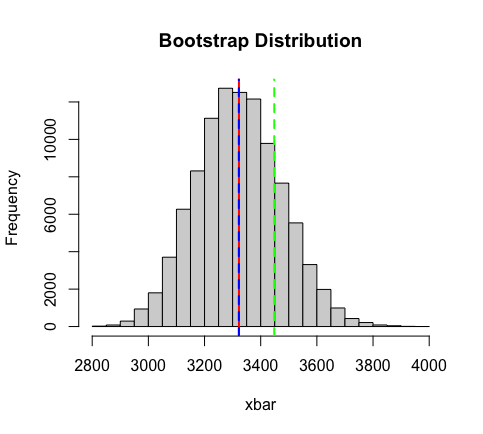
\includegraphics[width=0.5\tw]{11/fig-ncbirths2.png}
\end{center}

\vspace{-0.25in}

\textbf{\colorb{Bootstrap Center}}  $= 3322.2$g \\
\textbf{Bootstrap Standard Error}   $= 151.98$g\\
\\
\\ 
\textbf{Bias} $=$ \textbf{\colorb{Bootstrap Center}} $-$ \textbf{\colorr{Sample Mean}}\\
\textbf{Bias} $= 3322.2--3322.5=-0.3$g \\
\\
\\
\textbf{Actual Population Mean} $= 3448.26$g\\
\textbf{CLT SE} $= \frac{\mbox{sd(NCBirths2004\$Weight)}}{\sqrt{10}}= 154.2357$g\\
\end{multicols}

%\[ \mbox{index} = \left( \begin{array}{c} 463 \\ 346 \\ 2 \\ \vdots \\ 5 \\ 1004 \end{array} \right) 

\pagebreak

\pagebegin{Comparing CLT with Bootstrapping}

Consider the theoretical population $X \sim N(23,7)$. Below we compare the sampling distribution for the mean obtained using the central limit theorem on the top row with one random sample and a corresponding bootstrap distribution for the sample mean on the bottom row\footnote{See file Chap5-Compare.R for code that created the figure}..

\begin{center}
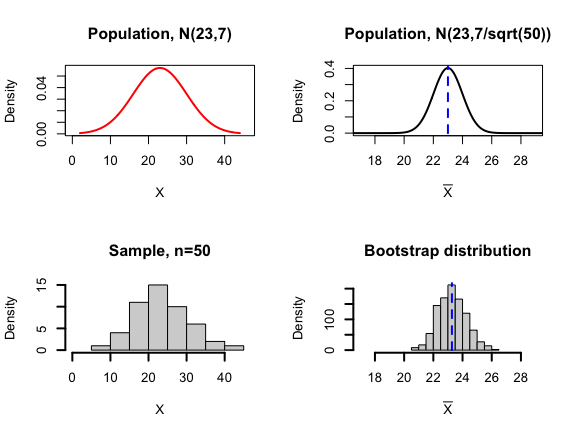
\includegraphics[width=0.75\tw]{11/fig-compare2.png}
\end{center}

\begin{center}
\begin{tabular}{lll}
\hline
 & Mean \ \ \ \ \ \ \ \ \ \ & Standard deviation \\
 \hline
Population & 23 & 7 \\
Theoretical Sampling Dist for $\bar{X}$ \ \ \ \ \ \ \ \ \ \ & 23 & $0.99$ \\
Sample ($n=50$) & $23.14$ & $6.69$ \\
Bootstrap distribution & $24.15$ & $0.92$\\
\hline
\end{tabular}
\end{center}


\bb[resume]
\ii Compare the population and sample distributions. What is similar about the two distributions? What are the differences? \vfill

\ii Compare the sampling distribution and bootstrap distribution. What is similar about the two distributions? What are the differences?
\vfill
\ee

\clearpage

\pagebegin{The Plug-in Principle}

 \bbox
\textbf{\colorb{The Plug-in Principle:}} If something (such as a characteristic of a population) is unknown, substitute (plug-in) an estimate.\medskip

Bootstrapping is an extreme application of this principle. We replace the entire popluation (not just one parameter with one value) by the entire set of data from the sample.
\ebox

\bbox
\bi
\ii The goal of a bootstrap distribution is to estimate a sampling distribution for some statistic.
\ii Bootstrap distributions are \textbf{\colorr{biased estimators for the center}} of a sampling distribution since they are centered near $\bar{x}$ not necessarily $E(\overline{X}) = \mu$. %\medskip
\ii Thus the center of a bootstrap distribution is not useful alone, but they are useful at quantifying the behavior of a parameter estimate. % \medskip
\ii For most common statistics, bootstrap distributions provide good estimates for the true \textbf{\colorb{spread}}, \textbf{\colorb{shape}}, and \textbf{\colorb{bias}} of a sampling distribution.
\ei
\ebox

\bb[resume]
\ii Arsenic is a naturally occurring element in the groundwater in Bangladesh. Much of this water is used for drinking in rural areas,
so arsenic poisoning is a serious health issue. The dataset\footnote{http://www.bgs.ac.uk/arsenic/bphase2/datadownload.htm} \textit{\textbf{\colorb{Bangladesh}}} contains measurements on arsenic, chlorine, and cobalt levels (in parts per billion, ppb) present in each of 271 groundwater samples.\label{q:arsenic}

Open the R Markdown file \href{https://ucdenver.instructure.com/files/14966546}{\colorb{Chap5-Bootstrap-Part1.Rmd}} to answer the questions. 


\bb
\ii What are the mean and standard deviation of the arsenic level of the sample? Use correct notation when expressing each value. \vfill
\ii Create a histogram to show the shape of the distribution of the sample data. How would you describe the shape? \vfill
\ii Create a boostrap distribution for the sample mean by generating $10,000$ bootstrap resamples. Plot the results on a histogram. \vfill
\ii Describe the center, shape and spread of the bootstrap distribution. \vfill
\ee
\ee

%%%%%%%%%%%%%%%%%%%%%%%
%% Stuff  below removed since not needed!
%%%%%%%%%%%%%%%%%%%%%%%

%\clearpage

%\begin{multicols}{2}
%library(resampledata)\\
%\\
%Arsenic $<-$ Bangladesh$\$$Arsenic\\
%sample.mean $<-$ mean(Arsenic)\\
%sample.sd $<-$ sd(Arsenic)\\
%\\
%hist(Arsenic)\\
%\\
%n $<-$ length(Arsenic) \# how many observations in Arsenic\\
%N $<- 10^4$ \# Number of bootstrap samples\\
%boot.mean $<-$ numeric(N)\\
%for (i in 1:N)\\
%$\left\{ \right.$\\
%\indent  \ \ \ \ \ x $<-$ sample(Arsenic, n, replace = TRUE)\\
%\indent  \ \ \ \ \ boot.mean$\lbrack i \rbrack  <-$ mean(x)\\
%$\left. \right\}$\\
%\\
%hist(boot.mean, xlab = "xbar",  \\
%\indent \ \ \ \ \ main = "Bootstrap Distribution")\\
%abline(v = sample.mean, col = "red", lwd = 2, lty = 2)\\

%\columnbreak

%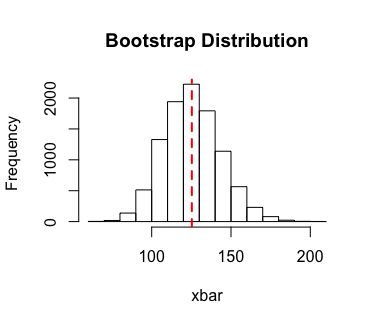
\includegraphics[width=0.5\tw]{11/fig-arsenic.png}
%\end{multicols}

%\clearpage

%\bbox
%If $X_1, X_2, \ldots , X_n$ are random variables from a distribution with parameter $\theta$ and $g(X_1, X_2, \ldots , X_n)$ an
%expression used to estimate $\theta$, then we call this function an \textbf{\colorb{estimator}}. For most common estimators, the following hold:
%\bi
%\ii The \textbf{\colorr{center}} of the bootstrap distribution is NOT an accurate approximation for the center of the sampling distribution.
%\ii The \textbf{\colorb{spread}} of the bootstrap distribution DOES reflect the spread of the sampling distribution.
%\ii The \textbf{\colorb{skewness}} of the bootstrap distribution DOES reflect the skewness of the sampling distribution.
%\ii The bootstrap distribution CAN be used to estimate the \textbf{bias} of the sampling distribution.
%\ei
%\ebox

%\bb[resume]
%\ii In the arsenic example, what is the parameter $\theta$ we are estimating? What is the estimator function $g(X_1, X_2, \ldots , X_n)$?  \vspace{1in}
%\ee

%\bb[resume]
%\ii Construct a bootstrap distribution for the sample mean with $10^4$ bootstrap samples, and compute the mean and
%standard error of the bootstrap distribution.

%\ii For a normal distribution, we know that 95\% of all values are within approximately 2 standard deviations from the mean. Using the quantile function find similar the cutoffs for the middle 95\% of all sample means in the arsenic bootstrap distribution. \vfill
%\ee

%\clearpage

%\pagebegin{Section 5.3: Bootstrap Percentile (Confidence) Intervals}


%%%%%%%%%%%%%%%%%%%%%%%
%% Stuff  below removed since ran out of times
%%%%%%%%%%%%%%%%%%%%%%%%%

%\pagebegin{Bootstrap Interval Estimates}

%Usually when estimating an unknown population parameter, we give an \textbf{\colorb{interval estimate}} that gives range of plausible values for the parameter by accounting for the uncertainty due to the variability in sampling.


%\begin{center}
%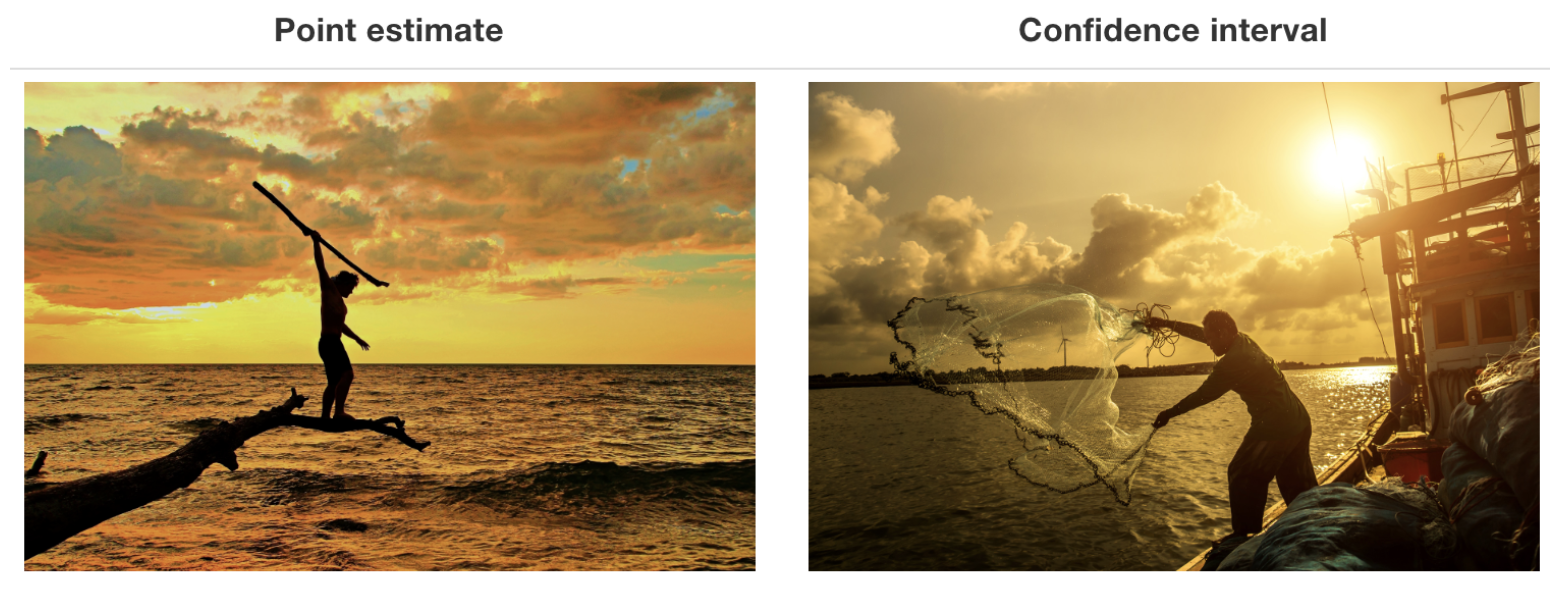
\includegraphics[width=0.75\tw]{11/fig-fishing.png}
%\end{center}

%\bbox
%The interval between the $2.5$ and $97.5$ percentiles of the bootstrap distribution of a statistic is a \textbf{\colorb{95\% bootstrap percentile confidence interval}} for the corresponding parameter.

%\bi
%\ii If most of the sample statistics are located in a certain interval of the bootstrap distribution, it seems plausible the true value of the parameter is in this interval!
%\ii We would say we are 95\% confident that the interval contains the actual value of  the population parameter.
%\ei
%\ebox

%\bb[resume]
%\ii We return the bootstrap distribution we created to approximate the sampling distribution for the mean arsenic level of groundwater in Bangladesh in question\ref{q:arsenic}.
%\bb
%\ii Following the process above, compute a 95\% bootstrap percentile confidence interval for the mean arsenic level in groundwater in Bangladesh. \vfill 

%\ii Interpret the practical meaning of the interval. \vfill

%\ii Sometimes it is nice to describe the interval as a value plus or minus some margin of error. Recall with normal distributions, approximately 95\% of the data is within 2 standard deviations of center of the distribution.  Construct a symmetric 95\% bootstrap confidence interval for the mean arsenic level.  \vfill
%\ee

%\clearpage

%\ii We return to the mean weight of newborns in North Carolina in question\ref{q:newborn}. Answer the questions below assuming the population is all newborns in North Carolina in 2004 (which is unknown), and we have one large random sample size $n=1009$ in the dataset \textit{\textbf{\colorg{NCBirths2004}}}.

%\bb
%\ii Give a 95\% bootstrap percentile confidence interval for the mean weight of babies born in North Carolina in 2004.\vfill %See \textbf{NCBirths.R}.

%\ii Give a 90\% bootstrap percentile confidence interval for the mean weight of babies born in North Carolina in 2004. \label{q:90per} \vfill

%\ii Interpret the practical meaning of your 90\% bootstrap percentile confidence interval in question \ref{q:90per}. \vfill

%\ii When we decreased the confidence level, what happend to the confidence interval estimate? \vfill
%\ee
%\ee

